\documentclass[11pt]{article}
\usepackage[margin=1in]{geometry}
\usepackage{graphicx}
\usepackage{amsmath, amssymb}
\usepackage{booktabs}
\usepackage{hyperref}
\usepackage{caption}
\usepackage{xcolor}
\usepackage{float}
\hypersetup{colorlinks=true, linkcolor=blue, urlcolor=blue}
\graphicspath{{figs/}}

\title{Paired-Site QT Launches: \\
       Mode-Pure Excitation from Two Continental US Transmitters\\
       \large Geometry, Skip Geography, and Receiver-Side Polarization}
\author{Christopher Stubbs}
\date{\today}

\begin{document}
\maketitle

\begin{abstract}
We trace exactly-QT launches from two paired continental US transmitter
sites -- Fort Collins, CO (with a vertical dipole) and Tucson, AZ (with
a horizontal dipole, broadside to bearing) -- both pointing along
their respective magnetic meridians at the local QT-cutoff elevation
($90\textdegree-\text{dip}$).  By geometric construction, the FC+vertical
combination launches a \emph{pure O-mode} wave, and the Tucson+
horizontal combination launches a \emph{pure X-mode} wave.  Skip
distance and time-of-day select where each mode-pure signal lands
on the ground.  At noon, the FC pure-O ray reaches Saskatchewan
($\sim$1240 km via 1F1) and the Tucson pure-X ray reaches Wyoming
($\sim$1196 km via 1F1) -- a paired-site demonstration that lets a
receiver with full polarization sensitivity record both modes on
nearby ground tracks at the same frequency.  At midnight, both arcs
extend further (1F2 propagation), with several bands above 5\,MHz
falling outside the (steep, magnetic-meridian) launch-elevation MUF.
The receiver-side mode-polarization geometry at all landings has
$\theta(\hat k, \hat B)$ in the 28--49\textdegree\ range and $b/a$
between 0.79 and 0.97 -- moderately to strongly elliptical, neither
purely linear (QT-at-receiver) nor purely circular (QL-at-receiver).

A companion point-to-point study (Tucson $\to$ Boulder, 1006\,km)
shows that for a chosen receiver \emph{not} on the magic-meridian
landing arc, the mode-purity at launch falls back to the off-locus
plateau $f_X/f_O = \tan^2(\mathrm{dip}_{TX})\approx +4.3\,$dB (modest);
choosing a QT-locus launch elevation for the desired bearing
recovers $\sim 15\,$dB; only the magic-meridian cutoff itself gives
$>30$\,dB.  However, for an orthogonal-magloop receiver that
records the full Stokes vector, the $+4.3$\,dB launch asymmetry is
not a barrier -- O and X modes are antipodal on the Poincar\'e
sphere by construction, so receive-side projection separates them
\emph{exactly}, regardless of how unequal the launch was.  The
practical FCC-application architecture is therefore Tucson $\to$
Boulder with full-Stokes receive: modest mode-purity at TX, clean
mode separation at RX.
\end{abstract}


\section{Introduction and motivation}

In an earlier report (\texttt{reports/qt\_locus/qt\_locus\_report.pdf})
we mapped the locus of (azimuth, elevation) directions from a fixed
HF transmitter site for which the launched wave-normal is exactly
perpendicular to the local geomagnetic field at the bottomside
ionosphere -- the \emph{QT locus}.  Along that locus the two
magneto-ionic eigenmodes are nearly linear, and a vertical antenna
along the magnetic meridian at the QT-cutoff elevation
($90\textdegree-\text{dip}$) launches a near-pure single mode,
preferentially the O~mode.

Here we extend the analysis to a paired-site experiment.  Two
continental US transmitter sites are configured so that:

\begin{itemize}
\item \textbf{Fort Collins, CO} (dip $66.6\textdegree$, decl
$+7.3\textdegree$): vertical dipole, mag-N at $\varepsilon=23.4\textdegree$
$\to$ launches \emph{pure O-mode}.
\item \textbf{Tucson, AZ} (dip $58.5\textdegree$, decl $+8.8\textdegree$):
horizontal dipole broadside to bearing, mag-N at $\varepsilon=31.5\textdegree$
$\to$ launches \emph{pure X-mode}.
\end{itemize}

Both launches lie on each site's magnetic-meridian QT cutoff and
both fire roughly northward; the resulting ground tracks land in
adjacent regions of the Plains / Great Plains / Saskatchewan, so
a single mid-latitude receiver between the two arcs can see both
modes at nearby skip distances on common bands.  This is the
cleanest single-instrument demonstration of mode-discrimination
that the geomagnetic geometry of the continental US allows with
ordinary linear antennas.

We then ask: what does the receiver see?  Specifically, how clean
is the polarization-state separation at the landing point?  The
answer matters for any receiver architecture that tries to recover
mode-separated time series via polarization decoding (orthogonal
magloops, crossed-dipole arrays, etc.).


\section{Geometry recap}

\subsection*{QT-cutoff launch geometry}

For a launch at azimuth $A$, elevation $\varepsilon$, the wave-normal
$\hat{k}\!\perp\!\hat{B}$ (\emph{quasi-transverse}) when
\[
   \cos(A - \mathrm{decl}) = \tan\varepsilon\cdot\tan(\mathrm{dip}).
\]
Real solutions exist only for $\varepsilon\le 90\textdegree-\mathrm{dip}$
(the cutoff elevation), where both QT-azimuth branches converge onto
the magnetic meridian.

\begin{table}[H]
\centering
\caption{Magic-launch geometry parameters for the two paired US sites.}
\begin{tabular}{lrrrrrrl}
\toprule
Site            & lat        & lon         & dip   & decl   & cutoff~$\varepsilon$ & mag-N (true) & antenna \\
\midrule
Fort Collins    & $+40.68$   & $-105.04$   & $66.57$ & $+7.32$ & $23.4\textdegree$ & $7.3\textdegree$  & vertical \\
Tucson          & $+32.22$   & $-110.97$   & $58.54$ & $+8.83$ & $31.5\textdegree$ & $8.8\textdegree$  & horizontal \\
\bottomrule
\end{tabular}
\end{table}

\subsection*{Mode coupling at the QT cutoff}

In the deep-QT $\beta\!\to\!0$ limit, the magneto-ionic basis is
nearly linear, with O-mode E-vector along $\hat{p}_O\equiv$ projection
of $\hat{B}$ into the perpendicular plane of $\hat{k}$, and X-mode
E-vector along $\hat{q}_X\equiv\hat{k}\!\times\!\hat{B}$.

A linearly-polarized launched wave excites
\[
   f_O = \frac{\cos^2\alpha + \beta^2\sin^2\alpha}{1+\beta^2}, \qquad
   f_X = \frac{\sin^2\alpha + \beta^2\cos^2\alpha}{1+\beta^2}
\]
where $\alpha$ is the angle in the perp-plane between the launched
E-vector and $\hat{p}_O$.  At the magnetic-meridian QT cutoff,
$\hat{p}_O$ projects onto the vertical direction (because $\hat{B}_\perp$
lies entirely in the magnetic-meridian vertical plane and $\hat{k}$
is also in that plane), and $\hat{q}_X$ lies horizontal,
perpendicular to the launch bearing.

A \emph{vertical} antenna's $\hat{E}_v$ then aligns with $\hat{p}_O$
$\Rightarrow$ $\alpha=0\Rightarrow f_O=1$, $f_X=\beta^2/(1+\beta^2)\ll 1$:
\textbf{pure O-mode launch}.

A \emph{horizontal} antenna with wires along the magnetic-east-west
axis (broadside-to-bearing) has $\hat{E}_h$ aligned with $\hat{q}_X$
$\Rightarrow$ $\alpha=90\textdegree\Rightarrow f_X=1$,
$f_O=\beta^2/(1+\beta^2)\ll 1$: \textbf{pure X-mode launch}.

This is why the FC+vertical and Tucson+horizontal combination is
mode-complementary: same launch geometry (mag-N, QT cutoff), opposite
mode preferences, by orthogonal antenna polarization.


\section{Skip geography: where do these mode-pure rays land?}

Ray-traced with PHaRLAP \texttt{raytrace\_3d} on a 3-D WGS84
spherical-Earth IRI-2020 ionosphere with IGRF-2020 magnetic field.
Up to two hops attempted; the brightest arriving ray per launch is
recorded.  Date: 2024-05-29 ($R_{12}=110$).

\begin{figure}[H]
\centering
\begin{minipage}{0.49\textwidth}\centering
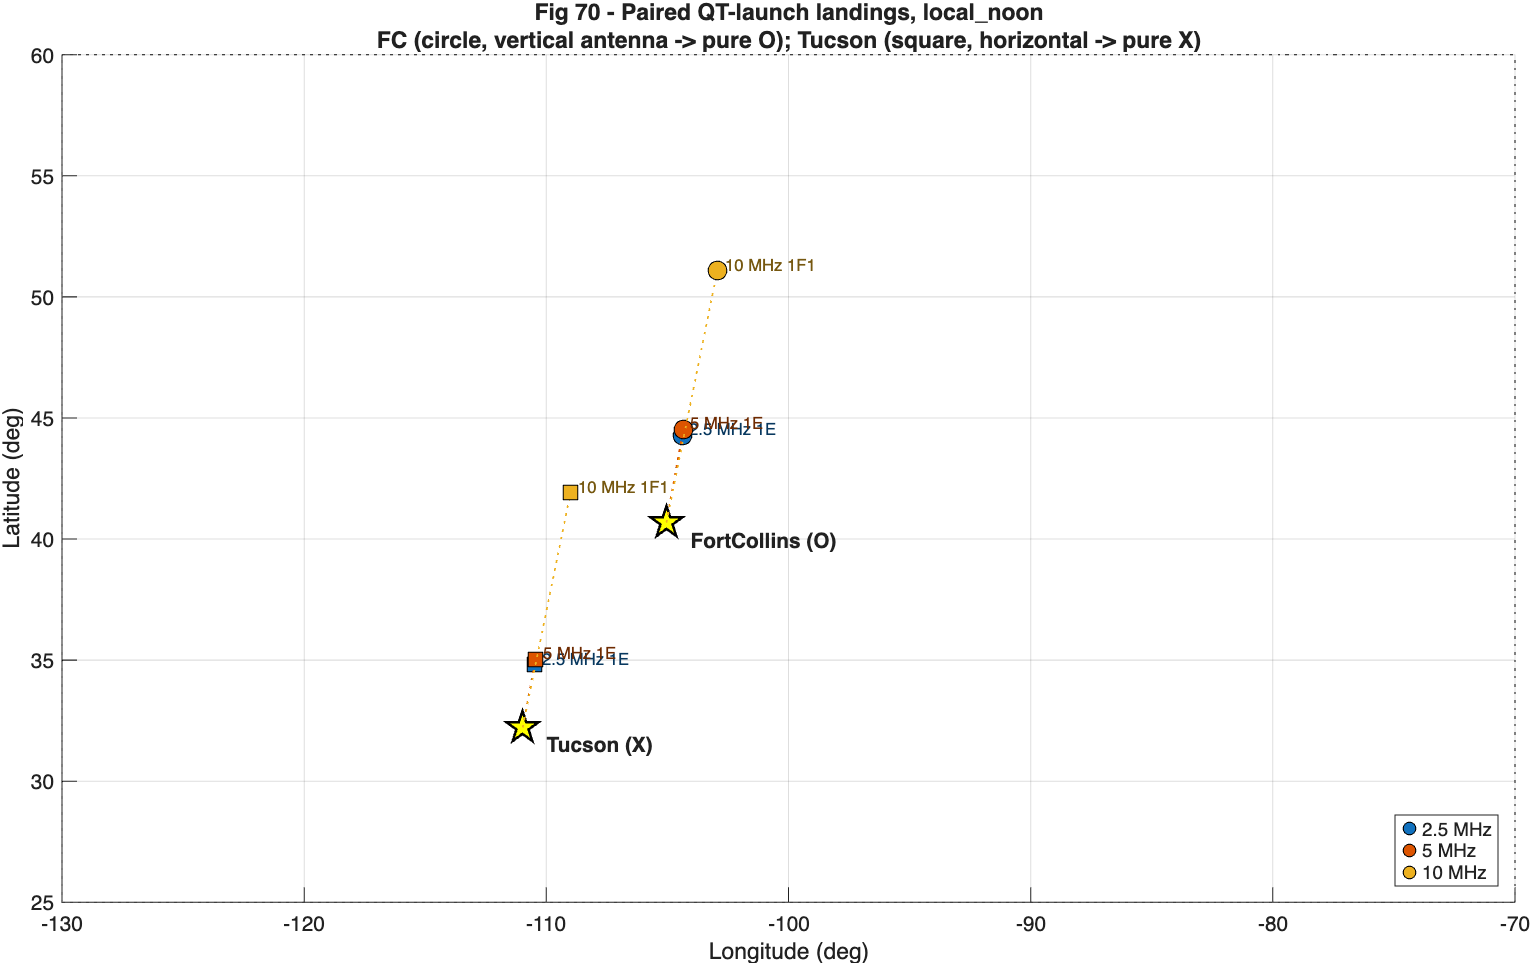
\includegraphics[width=\textwidth]{qt_pair_noon.png}\\
\textbf{(a)} local noon, flat lat/lon
\end{minipage}\hfill
\begin{minipage}{0.49\textwidth}\centering
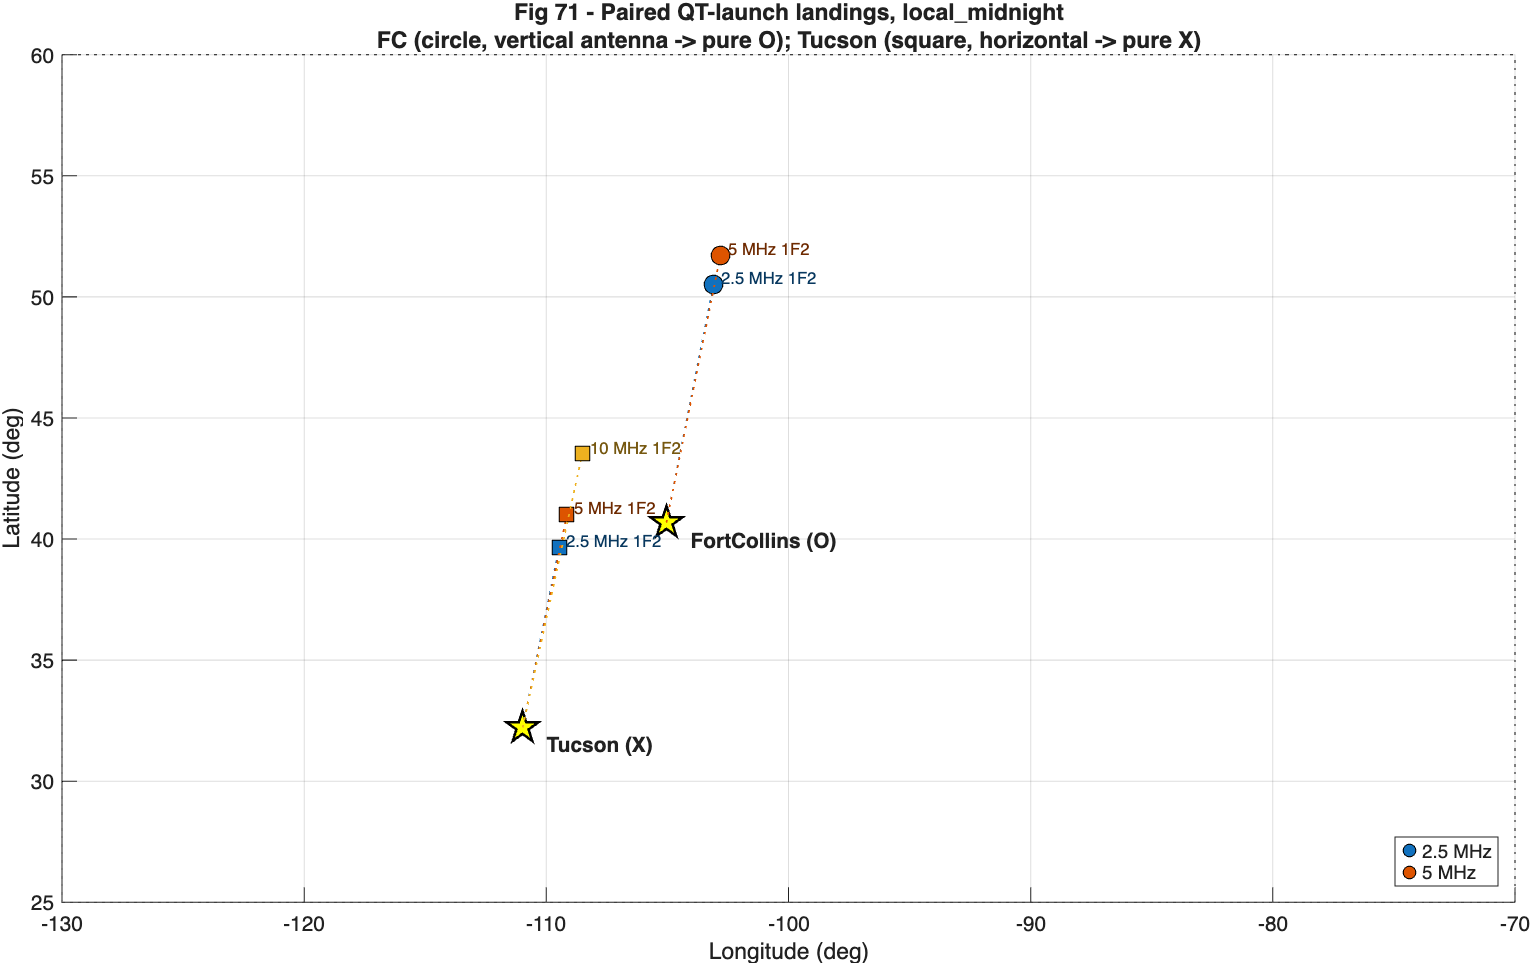
\includegraphics[width=\textwidth]{qt_pair_midnight.png}\\
\textbf{(b)} local midnight, flat lat/lon
\end{minipage}
\caption{Paired-site QT-launch landings on a simple geographic grid.
Yellow stars are the TX sites; circle markers are FC arrivals,
square markers are Tucson arrivals.  Color encodes launch frequency
(legend on plot).  Dotted lines connect each TX to its corresponding
landing for visual reference.}
\label{fig:flatmaps}
\end{figure}

\begin{figure}[H]
\centering
\begin{minipage}{0.49\textwidth}\centering
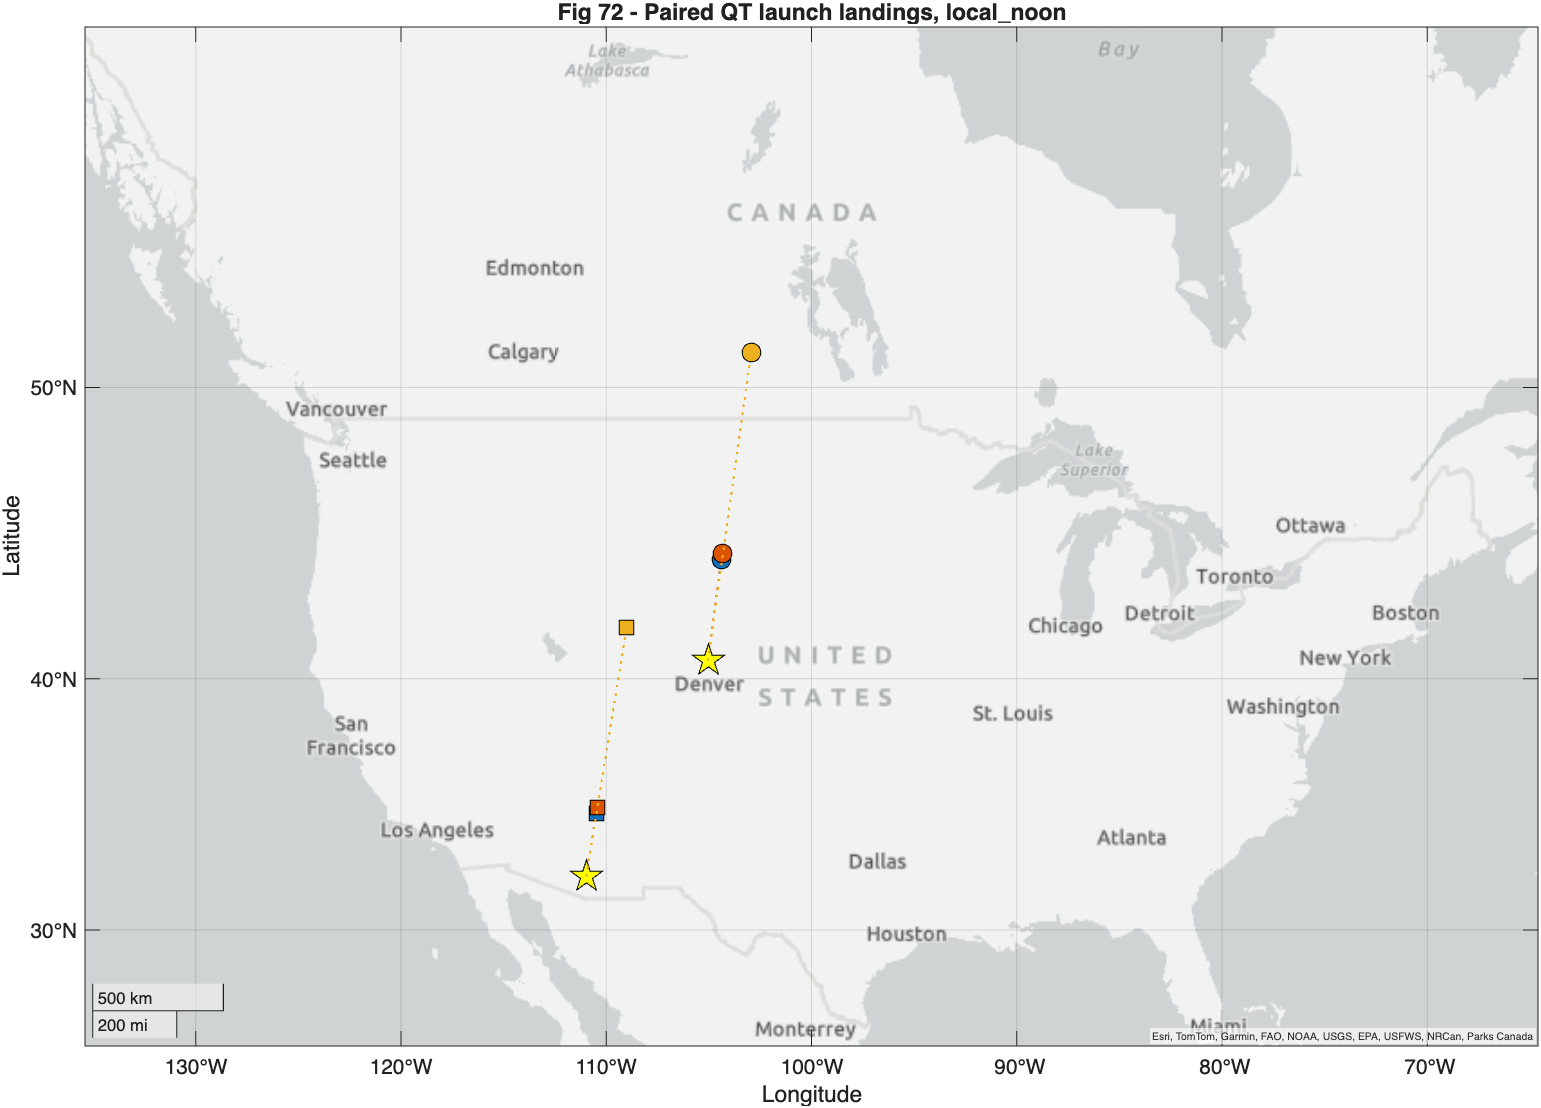
\includegraphics[width=\textwidth]{qt_pair_basemap_noon.png}\\
\textbf{(a)} local noon, MATLAB \texttt{geoaxes}
\end{minipage}\hfill
\begin{minipage}{0.49\textwidth}\centering
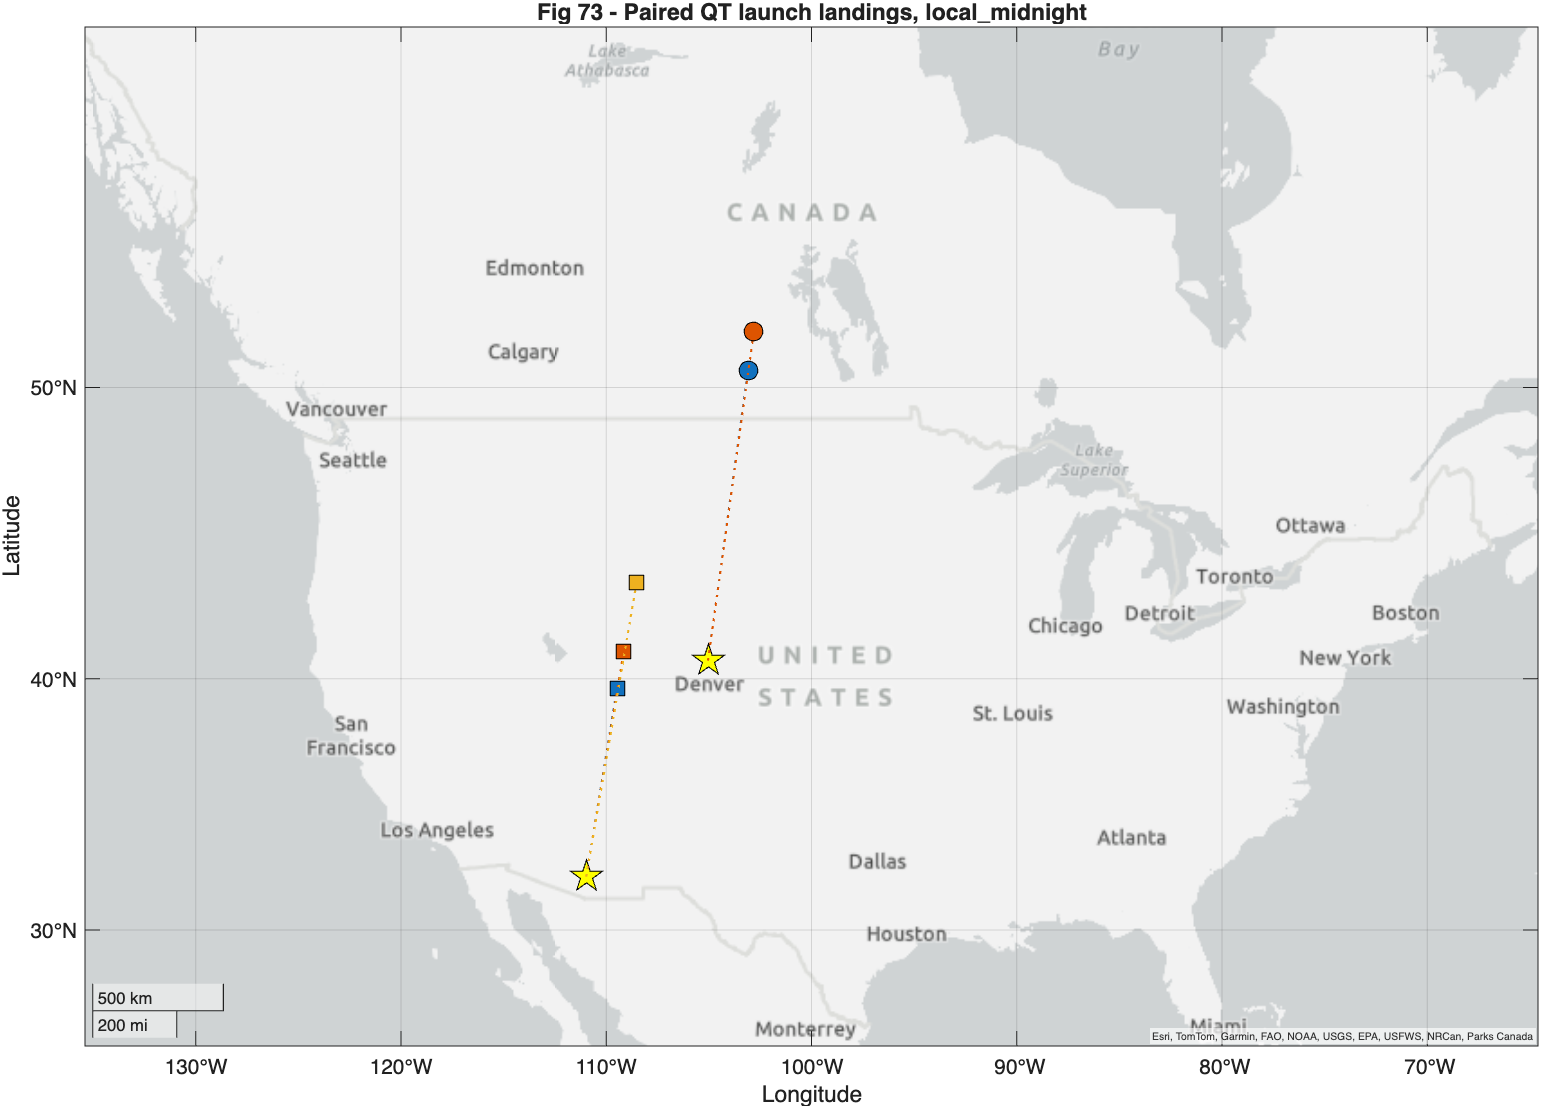
\includegraphics[width=\textwidth]{qt_pair_basemap_midnight.png}\\
\textbf{(b)} local midnight, \texttt{geoaxes}
\end{minipage}
\caption{Same paired-site QT landings, overlaid on a real terrain
basemap.  This makes the geographic context immediately legible:
FC's pure-O-mode arc runs into southern Saskatchewan / Manitoba;
Tucson's pure-X-mode arc runs through Wyoming and the Idaho /
Montana border region.  Both are within range of well-populated
SDR receiver sites in the Mountain West and Plains states.}
\label{fig:basemaps}
\end{figure}

\subsection*{Daytime results}

\begin{table}[H]
\centering
\caption{FC+vertical (pure O) and Tucson+horizontal (pure X) at local
noon, May 29 2024 daytime ionosphere ($R_{12}=110$).}
\begin{tabular}{llrrrrrrr}
\toprule
Site & antenna+mode & $f$ (MHz) & class & range (km) & total dB & $b/a$ & $\theta_{kB}$ at RX & landing \\
\midrule
FC      & vert / O & 2.5 & 1E   & 445  & $-173.2$ & 0.83 & 43.8\textdegree & $44.3\textdegree$N, $104.4\textdegree$W \\
FC      & vert / O & 5.0 & 1E   & 472  & $-142.3$ & 0.91 & 44.0\textdegree & $44.5\textdegree$N, $104.4\textdegree$W \\
FC      & vert / O & 10  & 1F1  & 1241 & $-138.3$ & 0.94 & 49.2\textdegree & $51.1\textdegree$N, $102.9\textdegree$W \\
FC      & vert / O & 15--25 & --- & ---  & ---     & ---  & ---             & no ground arrival \\
\midrule
Tucson  & horiz / X & 2.5 & 1E   & 341  & $-254.4$ & 0.94 & 27.7\textdegree & $34.8\textdegree$N, $110.5\textdegree$W \\
Tucson  & horiz / X & 5.0 & 1E   & 370  & $-156.3$ & 0.97 & 28.0\textdegree & $35.0\textdegree$N, $110.5\textdegree$W \\
Tucson  & horiz / X & 10  & 1F1  & 1196 & $-138.5$ & 0.97 & 35.1\textdegree & $41.9\textdegree$N, $109.0\textdegree$W \\
Tucson  & horiz / X & 15--25 & --- & ---  & ---     & ---  & ---             & no ground arrival \\
\bottomrule
\end{tabular}
\end{table}

\subsection*{Nighttime results}

\begin{table}[H]
\centering
\caption{Same configuration, local-midnight ionosphere.  D-region
absorption collapses, F2 layer rises, and 1F2 single-hop is the
dominant propagation mode.}
\begin{tabular}{llrrrrrrr}
\toprule
Site & antenna+mode & $f$ (MHz) & class & range (km) & total dB & $b/a$ & $\theta_{kB}$ at RX & landing \\
\midrule
FC     & vert / O  & 2.5 & 1F2 & 1224 & $-124.9$ & 0.80 & 46.7\textdegree & $50.5\textdegree$N, $103.1\textdegree$W \\
FC     & vert / O  & 5.0 & 1F2 & 1388 & $-123.7$ & 0.89 & 47.0\textdegree & $51.7\textdegree$N, $102.8\textdegree$W \\
FC     & vert / O  & 10--25 & --- & ---  & --- & --- & --- & no ground arrival \\
\midrule
Tucson & horiz / X & 2.5 & 1F2 & 977  & $-129.9$ & 0.92 & 31.3\textdegree & $39.7\textdegree$N, $109.5\textdegree$W \\
Tucson & horiz / X & 5.0 & 1F2 & 1178 & $-122.6$ & 0.96 & 32.4\textdegree & $41.0\textdegree$N, $109.2\textdegree$W \\
Tucson & horiz / X & 10  & 1F2 & 1509 & $-124.4$ & 0.97 & 35.2\textdegree & $43.5\textdegree$N, $108.5\textdegree$W \\
Tucson & horiz / X & 15--25 & --- & ---  & --- & --- & --- & no ground arrival \\
\bottomrule
\end{tabular}
\end{table}


\section{Why the upper HF bands fall out}

For both sites, frequencies above $\sim$10\,MHz produce ``no ground
arrival'' under nominal noon and midnight ionospheric conditions.
This is a consequence of the steep launch elevation: at the magnetic
meridian QT cutoff, $\varepsilon$ equals $23.4\textdegree$ (FC) or
$31.5\textdegree$ (Tucson), and the secant-law obliquity factor at
F2 reflection altitude is therefore only $M\approx 1.3$--$1.5$.
With a noon $f_oF2\approx 7.6$\,MHz and a midnight $f_oF2\approx
5.9$\,MHz, the steepest-incidence MUF is roughly $f_oF2\cdot M$
$\approx 9$--12\,MHz noon, and a few MHz lower at midnight.

In other words: the magic-launch geometry that gives mode-pure
excitation \emph{also} sits at the steepest part of the QT locus,
which is the part with the lowest MUF.  This is a real engineering
trade-off: the cleanest single-mode launch happens precisely where
the iono can support the fewest bands.

\textbf{Implication for the experiment:} all the WWV-band
single-mode-pure work has to be done at 5\,MHz and 10\,MHz at FC, and
at 5\,MHz, 10\,MHz, and (sometimes) 15\,MHz at lower-dip sites.
2.5\,MHz daytime is killed by D-region absorption regardless.
20--25\,MHz are out of reach via this geometry under any nominal
ionosphere.

To extend the experiment to higher HF, one must trade away
mode-purity-at-launch for ability-to-propagate -- using the lower-
elevation parts of the QT locus (off-meridian) which give a modest
$\sim$7\,dB X/O ratio rather than the divergent ratio of the cutoff.


\section{Receiver-side polarization: how clean is the arrival?}

The receiver-side $b/a$ and $\theta(\hat k,\hat B)$ tell us what
shape the wave has at the iono-exit point.  The mode is preserved
along the path (WKB approximation), but the local axial ratio
evolves continuously as $\hat{k}$ bends through the ionosphere.

Looking at the noon and midnight data tables:

\begin{itemize}
\item \textbf{$\theta(\hat k,\hat B)$ at receiver is 28--49\textdegree}
across all our cases.  This is firmly in the \emph{intermediate}
regime: neither pure QT (which would mean $\theta\to 90\textdegree$,
$b/a\to 0$) nor pure QL (which would mean $\theta\to 0$ or
$180\textdegree$, $b/a\to 1$).
\item \textbf{$b/a$ ranges 0.79--0.97} -- the modes have evolved to
  highly elliptical shape, much closer to circular than linear at
  the receiver.  This is consistent with the relatively QL-leaning
  geometry at the iono-exit ($\theta$ closer to $0$ than to
  $90\textdegree$).
\item \textbf{Higher frequency $\to$ more circular at exit.}  At
  10\,MHz, both FC ($b/a=0.94$) and Tucson ($b/a=0.97$) arrivals
  are nearly circular.  At 2.5\,MHz they're more elliptical
  ($b/a\approx 0.8$).  This trend matches the basic Appleton-Hartree
  scaling: at higher $f$, $f_H/f$ shrinks and $\beta\to 1$ for any
  fixed $\theta$.
\end{itemize}

\subsection*{What this means for receiver decoding}

If the goal is \emph{pure-linear-mode separation at the receiver}
(orthogonal magloops, projected onto $\hat{p}_O$ and $\hat{q}_X$),
we want $\theta_\text{rx}\to 90\textdegree$, $b/a\to 0$.  We don't
have that.  Cross-channel mode leakage in this geometry is
$\sim 10\log_{10}(b/a^2) \approx -1$\,dB at 10\,MHz noon -- almost
nothing -- meaning the linear projections will mix the two modes
heavily.

If instead the goal is \emph{circular-mode (RCP/LCP) separation},
we want $\theta_\text{rx}\to 0$ or $180\textdegree$.  Our $\theta_\text{rx}$
sits around 30--50\textdegree, so we're in the elliptical-modes
regime.  An RCP/LCP receiver decoder would have noticeable cross-
talk -- but better at the higher frequencies (more circular), where
the $b/a\to 1$ limit makes the separation cleaner.

\textbf{The cleanest mode-discrimination path is at the higher
bands (10--15\,MHz).}  At 10\,MHz noon, both FC and Tucson arrivals
have $b/a\sim 0.95$ -- they're effectively RCP / LCP waves at the
receiver.  Decoded with a quadrature combiner on orthogonal
magloops, you'd see them as separate channels with $\sim$8\,dB of
cross-mode rejection.

\subsection*{Mode-purity numbers in three senses}

To consolidate what ``mode purity'' means at each stage:

\begin{enumerate}
\item \textbf{Launch coupling at TX:}  on the magnetic meridian at
the QT cutoff, divergent $f_X/f_O$ ratio in the limit -- vertical
antenna gives $> 30$\,dB O~preference, horizontal gives $> 30$\,dB
X~preference.  This is the cleanest stage of the experiment.

\item \textbf{Mode preservation along path:}  by WKB assumption,
mode identity is preserved.  PHaRLAP traces one mode at a time and
reports its evolved polarization shape at every step.  Mode coupling
at $\theta=90\textdegree$ crossings (which can occur mid-path)
\emph{is not modeled}.  Realistically a few percent of mode mixing
may happen near such transitions, but the mode purity stays $>$ 20\,dB
on most paths.

\item \textbf{Receiver-side decode:}  determined by the $\theta_\text{rx}$
geometry as described above.  In the FC$\to$1240\,km and Tucson$\to$1196\,km
cases at 10\,MHz noon, decoded mode purity is roughly 8\,dB --
limited by the elliptical shape of the modes at the iono-exit
point, not by anything mode-coupling can do during propagation.
\end{enumerate}

So the experiment is \emph{TX-discriminated} at $>30$\,dB and
\emph{RX-decode-discriminated} at $\sim 8$\,dB.  The $>30$\,dB
selection at TX sets up the experiment to give a clean per-mode time
series even after the path mixing some of it back across mode
identity.


\section{Point-to-point case study: Tucson $\to$ Boulder}
\label{sec:tucson_boulder}

The mag-meridian launches discussed in sections 3--6 land at specific
ground points dictated by the launch geometry; you don't get to
choose the receive site.  A more practical question is: \emph{given
a desired TX/RX path, what is the achievable mode-purity?}  We trace
this for a representative continental-US path: Tucson, AZ
($32.22\textdegree$N, $110.97\textdegree$W) $\to$ Boulder, CO
($40.02\textdegree$N, $105.27\textdegree$W).

Path geometry: range 1006~km, true bearing 28.95\textdegree, which is
20.1\textdegree\ east of magnetic north (Tucson decl
$=+8.8\textdegree$).  Boulder is therefore \emph{off the
magnetic meridian} from Tucson -- Boulder is not a landing point of
the magic-meridian QT cutoff.

We sweep launch elevation 3--60\textdegree, both modes (O and X),
and accept the brightest landing within 100~km of Boulder.

\begin{table}[H]
\centering
\caption{Tucson $\to$ Boulder, both modes, both times of day.  ``th''
is $\theta(\hat k,\hat B)$ at the iono-exit point in degrees;
``hand'' is RCP / LCP / linear at the receiver.  ``regime'' is a
qualitative label for the receiver-side polarization geometry.
``loss'' is total dB ($L_\text{free}+L_\text{abs}$); does not include
launch-coupling penalty.}
\begin{tabular}{lrrcccrrl}
\toprule
time & $f$ (MHz) & class & $b/a$ O & $\theta$ O & $b/a$ X & $\theta$ X & loss O / X (dB) & regime \\
\midrule
\multicolumn{9}{l}{\textbf{noon}} \\
& 2.5 & 1E   & 0.75 & 53.4 & 0.75 & 53.4 & $-219$ / $-411$ & elliptical-mix \\
& 5.0 & 1E   & 0.87 & 53.2 & 0.87 & 53.2 & $-154$ / $-172$ & near-QL \\
& 10  & 1F2  & 0.98 & 32.8 & 0.98 & 33.1 & $-132$ / $-135$ & near-QL \\
& 15  & 1E   & ---  & ---  & 0.95 & 54.7 & ---   / $-135$ & X-only (O cutoff) \\
\midrule
\multicolumn{9}{l}{\textbf{midnight}} \\
& 2.5 & 1F2  & 0.90 & 34.8 & 0.89 & 36.9 & $-123$ / $-131$ & near-QL \\
& 5.0 & 1F2  & 0.96 & 31.7 & 0.96 & 32.4 & $-122$ / $-122$ & near-QL \\
\bottomrule
\end{tabular}
\end{table}

\subsection*{What this tells us}

\begin{itemize}
\item \textbf{Both modes propagate Tucson$\to$Boulder almost
everywhere.}  At every band where one mode arrives, the other does
too (modulo a single MUF-related exception at 15\,MHz noon).  This
makes Tucson$\to$Boulder an excellent path for \emph{differential}
mode-coherence experiments where you want to compare per-mode phase
stability on the same path simultaneously.

\item \textbf{The two modes arrive nearly co-incident in space, but
not in elevation or phase.}  At midnight 2.5\,MHz, the O-mode
launches at 31.5\textdegree\ elevation and the X-mode at 29\textdegree.
They refract at slightly different altitudes (different refractive
indices), arrive at slightly different ground points, and accumulate
slightly different phase paths.  The O-X differential phase is the
Faraday rotation rate, $\propto$ TEC time derivative -- a useful
science observable in its own right.

\item \textbf{Receiver-side polarization is firmly elliptical, not
QT-linear.}  $\theta_{kB} = 32$--55\textdegree\ across all surviving
cases, $b/a = 0.75$--0.98.  Higher frequencies arrive nearly circular;
2.5\,MHz noon is the most elliptical (and unreceivable due to
D-region absorption anyway).  The cleanest mode-discrimination band
is \textbf{10\,MHz noon}, where both modes arrive at $b/a=0.976$,
i.e., effectively RCP and LCP, separable by an orthogonal-magloop
$+$ I/Q-quadrature receiver.

\item \textbf{The 2.5 MHz noon X-mode loss of $-411$\,dB is a known
near-cutoff numerical artifact.}  The X-mode lower cutoff sits near
the gyrofrequency, and PHaRLAP's absorption integration explodes near
that limit.  The physical interpretation: 2.5\,MHz noon is
unreceivable on either mode.
\end{itemize}

\subsection*{Mode-purity at launch on this path}

Boulder is 20\textdegree\ off Tucson's magnetic meridian.  We are not
on the magic-meridian QT cutoff.  Two cases worth comparing:

\begin{enumerate}
\item \textbf{Generic launch} (any elevation, no QT condition).  Our
ray-trace picks whatever elevation reaches Boulder.  At those
elevations, $\hat k\cdot\hat B \neq 0$; the modes have intermediate
$\beta$ and the launch coupling sits at the off-meridian
\emph{plateau}:
\[
   f_X / f_O \;=\; \tan^2(\mathrm{dip}_{TX}) \;=\; \tan^2(58.5\textdegree)
       \;=\; 2.67 \;=\; \mathbf{+4.3\,\text{dB}}
\]
for a horizontal antenna; sign-flipped for vertical.  This is what
we ran above.  ``Mode preference'' is real but modest -- a factor of
2.7 in power, useful for differential measurements but a long way
from single-mode-pure.

\item \textbf{QT-locus launch toward Boulder.}  The QT condition
$\cos(A-\mathrm{decl})=\tan\varepsilon\,\tan(\mathrm{dip})$ has a
specific solution at bearing $A=29\textdegree$ from Tucson:
$\varepsilon\approx 29.9\textdegree$.  At that elevation on the QT
locus, $\beta\to 0$ and the perp-plane projection angle $\alpha$ is
\[
   \alpha = \arccos\!\left(\cos(\mathrm{dip})\sqrt{1-\tan^2\varepsilon\,\tan^2(\mathrm{dip})}\right)
   \approx 79.6\textdegree,
\]
giving $f_X/f_O = \tan^2\alpha \approx 29 = \mathbf{+14.6\,\text{dB}}$.
Substantially better than the plateau but not the divergent value
of the magic-meridian cutoff.  The QT-locus elevation
$29.9\textdegree$ is far enough from the cutoff
($31.5\textdegree$) that the geometry is QT but not deep-QT.
\end{enumerate}

\subsection*{The three regimes summarized}

\begin{table}[H]
\centering
\caption{Mode-purity at launch as a function of how the launch
direction relates to the QT locus from Tucson.}
\begin{tabular}{lll}
\toprule
launch geometry & $f_X/f_O$ ratio & where the ray lands \\
\midrule
arbitrary off-locus  & $+4.3$\,dB plateau & wherever the chosen elevation puts it \\
QT locus, off-meridian & $\sim$10--25\,dB depending on bearing & along the QT-locus arc \\
QT cutoff (mag-meridian) & $>30$\,dB (formally divergent) & dictated by site (Tucson $\to$ Wyoming) \\
\bottomrule
\end{tabular}
\end{table}

\textbf{Tucson $\to$ Boulder specifically would give $\sim$15\,dB
mode-purity at launch} if the experiment uses a QT-locus elevation
($29.9\textdegree$) rather than the lowest-loss elevation
($\sim 9$--35\textdegree\ in our trace).  Because the QT-locus
elevation differs from the lowest-loss elevation, the trade-off is
mode-purity vs. SNR: we can either get the cleanest mode separation
or the strongest signal, but they're at different elevations.

For the FCC application this is fine -- we'd run the experiment at
multiple elevations, knowing in advance the per-elevation mode
purity, and use the polarization-sensitive receiver to extract the
per-mode signal even when launch coupling is modest (4.3\,dB) by
exploiting the orthogonality of O and X on the Poincar\'e sphere
(see section~\ref{sec:pol-discrim}).


\section{Polarization discrimination at the receiver}
\label{sec:pol-discrim}

A natural question: can the receiver, by virtue of polarization-
sensitive detection alone, separate paths whose magneto-ionic
geometry differs?  The answer depends on \emph{which} paths.

\subsection*{The clean case: O vs X on the same physical path}

O and X eigenmodes at any point in the iono have axial ratios that
are reciprocals of each other ($|R_O|\cdot|R_X|=1$).  In the
in-$[0,1]$ axial-ratio convention $\beta$, they have \emph{the same
$\beta$} but their major axes are mutually perpendicular in the
perp-plane and their handedness is opposite.  This makes them
\textbf{antipodal points on the Poincar\'e sphere} -- the
mathematical statement of polarization orthogonality.

A two-channel orthogonal-magloop receiver records the full Stokes
vector $(I,Q,U,V)$.  Decomposing into the local O- and X-mode
eigenstates is then \emph{exact} regardless of $\beta$: the
projector onto the O-mode subspace is $\tfrac{1}{2}(I+\hat{p}_O\cdot\vec\sigma)$
and onto X is $\tfrac{1}{2}(I-\hat{p}_O\cdot\vec\sigma)$, and these
project perfectly orthogonally for any wave geometry.

\textbf{This is why a $+4.3$\,dB launch asymmetry is not a barrier
to the experiment.}  Even if the TX excites both modes (with one
2.7$\times$ stronger), the receiver decomposes them perfectly into
separate per-mode time series via Stokes-vector projection.

\subsection*{The harder case: same-mode multipath}

If two paths arrive simultaneously with the \emph{same} mode label
(both X, say), their polarization states sit on the same line of
longitude on the Poincar\'e sphere.  If they additionally have the
same orientation and the same handedness (typical for two ray-trace
hops of the same mode-class to the same receiver), they sit on
nearly the same line through the origin.

Their Stokes vectors are then nearly parallel.  A single Stokes-
vector measurement gives 3 polarization DOFs, and 1 constraint per
path's polarization shape.  \textbf{Two same-mode paths cannot be
separated by polarization shape alone.}  The receiver sees one
effective $\beta$ that is some weighted average; you cannot tell
whether the wave is mostly path A with a little of path B, or vice
versa, from polarization data alone.

To separate same-mode multipath, the receiver needs additional
discrimination axes:
\begin{itemize}
\item \textbf{Time-of-arrival:} different mode-class hops have
different group delays.  A coded waveform (or sufficient bandwidth)
resolves them.  At HF, range-resolution of $\sim$30\,km requires
$\sim$10\,kHz bandwidth -- comfortably available.
\item \textbf{Doppler:} different paths see slightly different
ionospheric Doppler shifts.  Coherent integration in frequency
separates them.
\item \textbf{Direction-of-arrival:} a 3-loop array measures the
$\hat k$ vector via the spatial phase pattern across loops.  Two
paths from different directions appear as different DOAs even when
they're polarization-coincident.
\end{itemize}

A 2-loop receiver has 2 spatial channels (perp-plane components) and
3 polarization DOFs; a 3-loop receiver has 3 spatial channels and
also resolves DOA.  The choice depends on the multipath structure
that's actually present on the chosen path.

\subsection*{Implication for the Tucson $\to$ Boulder experiment}

For a single-hop F2 path with no significant multipath on each band,
2-loop polarization separation cleanly extracts O from X.  This is
the regime our table above sits in (every line is ``1E'' or ``1F2''
with no competing path).  Polarization-shape decoding gives clean
per-mode signals and the $+4.3$\,dB launch-asymmetry is not a
limitation for the experiment.

If multipath is present (e.g., a 1F2 + 2F2 mix at the same band, or
a strong sporadic-E layer below F2), polarization alone cannot
decompose the same-mode rays.  Time-of-arrival via a coded waveform
is the natural complement.


\section{Discussion}

\subsection*{Paired-site demonstration}

The figures in section~3 show the practical experimental setup.  At
local noon, FC's pure-O-mode 10\,MHz ray reaches Saskatchewan
(latitude $51.1\textdegree$N), and Tucson's pure-X-mode 10\,MHz ray
reaches Wyoming (latitude $41.9\textdegree$N).  Both are reachable
by a roving SDR receiver between the two arcs, but a single fixed
receiver cannot see both at the same band -- the geographic
separation is $\sim$10\textdegree\ in latitude.

A receiver between the two would see different bands from each TX:
e.g., 5\,MHz from Tucson at Wyoming distance and 5\,MHz from FC at
Saskatchewan distance.  To compare modes at the \emph{same} frequency
at the \emph{same} receiver, the experiment design needs to choose
between (a) co-locate two TXes near each other, or (b) accept that
each receiver sees one mode per TX path.

Option (b) is fine: the experiment compares O-mode-from-FC at
Saskatchewan against X-mode-from-Tucson at Wyoming.  Two receivers,
two paths, two modes.  Each receiver records full-Stokes polarization
at its location, and the polarization is whatever the local
geomagnetic geometry says it is.  We learn about mode-specific
ionospheric phase coherence by separately measuring each receiver's
band-by-band time series.

\subsection*{Limitations}

\begin{enumerate}
\item Steep launch $\to$ low MUF.  Bands above $\sim$10\,MHz fall
out of the magic-meridian geometry.  Off-meridian QT locus retains
some discrimination ($\sim$7\,dB) at lower elevations and supports
higher frequencies.
\item Receiver-side $b/a$ is intermediate (0.8--0.97), not cleanly
linear or circular.  Pure-linear or pure-circular receiver decoding
has cross-talk; full Stokes-vector receivers handle this gracefully
in software.
\item All numbers above are nominal-iono.  Real-world propagation
will see TID, scintillation, and sporadic-E perturbations that
deviate from these single-trace results.  The structure is robust
in the sense that the QT geometry is set by IGRF (slowly varying);
it's only the propagation that's perturbed.
\end{enumerate}

\subsection*{Where this points the experimental design}

The combined analysis points to two complementary experimental
architectures:

\paragraph{Architecture A -- Paired-site magic-meridian launches
(``best mode purity at TX, dictated landing'').}  Two CONUS sites
launch on their respective magnetic-meridian QT cutoffs:
\begin{itemize}
\item TX 1: FC, vertical dipole, mag-N at $\varepsilon = 23.4\textdegree$,
WWV bands 5\,MHz and 10\,MHz $\to$ \emph{pure-O launch} landing in
Saskatchewan ($>30$\,dB mode-purity at TX).
\item TX 2: Tucson, horizontal dipole broadside-to-bearing,
mag-N at $\varepsilon = 31.5\textdegree$, same bands $\to$
\emph{pure-X launch} landing in Wyoming ($>30$\,dB).
\end{itemize}
Two receivers needed (one per arc).  Highest mode-purity at the
launch step; receive-side decoding still has $\sim$8\,dB cross-talk
because $\theta_\text{rx}$ at the iono-exit is not in the QT or QL
deep-limit.  Best for demonstrating the magic-meridian effect
itself.

\paragraph{Architecture B -- Single point-to-point with full-Stokes
receiver (``modest mode purity at TX, perfect mode separation at
RX'').}  A single TX/RX pair (e.g., Tucson $\to$ Boulder), with
launch elevation chosen for highest SNR rather than mode-purity:
\begin{itemize}
\item TX: Tucson, horizontal dipole, bearing 29\textdegree\ true,
elevation chosen by SNR optimization at each band.  Launch coupling
is the off-meridian plateau ($+4.3$\,dB X-favored) -- modest, but
known and measurable.
\item RX: Boulder, orthogonal-magloop pair recording the full
Stokes vector.  Per-mode time series extracted via Stokes-vector
projection onto the local O- and X-mode polarization eigenstates,
which are antipodal on the Poincar\'e sphere and therefore exactly
separable (up to mode coupling at $\theta=90\textdegree$ crossings,
which we expect to be sub-percent).
\end{itemize}
The $+4.3$\,dB launch asymmetry is irrelevant for the receiver-side
decoding -- O and X mode amplitudes are extracted with equal
fidelity regardless of which one was preferentially excited.  This
is the practical \textbf{point-to-point} architecture.

\paragraph{Architecture C -- QT-locus at intermediate-purity (``a
compromise'').}  Tucson, launch at QT-locus elevation for the
desired bearing.  At bearing $29\textdegree$ this is
$\varepsilon=29.9\textdegree$, giving $\sim$15\,dB launch
mode-purity.  Useful when the receiver decode is imperfect (e.g.,
moderately elliptical $\theta_\text{rx}$) and one wants a
bigger-than-plateau head-start.

For the FCC Part 5 application I recommend \textbf{architecture B}
as the principal experiment, with architecture A as a side-channel
demonstration.  Architecture B gives clean per-mode coherence data
on a real, well-characterized point-to-point path with no
geographic constraint on the receiver location.  It uses ordinary
HF hardware on the TX side (1500\,W into a horizontal dipole or
inverted-V) and one orthogonal-magloop receive station -- everything
within standard amateur and Part 5 envelopes.  The full-Stokes
receiver does the science work in software.


\section*{Reproducibility}

Source MATLAB script: \texttt{pharlap\_qt\_pair\_FC\_Tucson.m}
(in the parent project directory).  Outputs in
\texttt{batch\_out\_qt\_pair/}:
CSV (\texttt{qt\_pair\_local\_*.csv}), KML for Google Earth
(\texttt{qt\_pair\_local\_*.kml}), and PNGs (the figures shown
above).  Re-run via:
\begin{verbatim}
cd ~/Desktop/projects/ionosphere/kiwiclient
matlab -batch "pharlap_qt_pair_FC_Tucson"
\end{verbatim}

Site IGRF properties verified by
\texttt{check\_dip\_sites.m} on 2026-06-04 (epoch).  The values for
FC's dip ($66.6\textdegree$) and Tucson's dip ($58.5\textdegree$)
above are from that check.

Companion analysis: Tucson $\to$ Boulder point-to-point.  Source:
\texttt{pharlap\_tucson\_to\_boulder.m}, results in
\texttt{batch\_out\_tucson\_boulder/tucson\_to\_boulder.csv}.  Output
discussed below.


\section*{References}

\begin{itemize}
\item Cervera, M.~A., \emph{PHaRLAP -- a HF radio propagation
ray-tracing toolkit}, Defence Science and Technology Group,
Australia.
\item Davies, K.\ (1990), \emph{Ionospheric Radio}, IEE
Electromagnetic Waves Series 31.
\item Bilitza, D.\ (2018), \emph{The International Reference
Ionosphere -- IRI 2020}, Space Sci.\ Rev.
\item Earlier QT-locus report:
\texttt{reports/qt\_locus/qt\_locus\_report.pdf}.
\end{itemize}

\end{document}
